\begin{figure}[ht]
    \centering


    \tikzset{every picture/.style={line width=0.75pt}} %set default line width to 0.75pt

    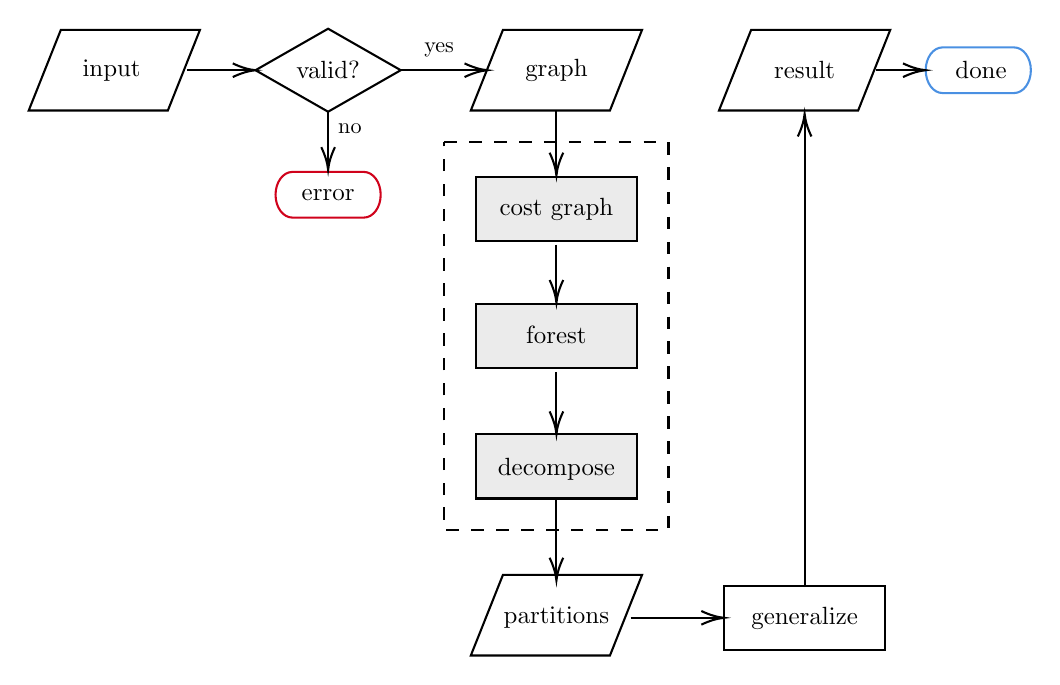
\begin{tikzpicture}[x=0.75pt,y=0.75pt,yscale=-1,xscale=1]
        %uncomment if require: \path (0,389); %set diagram left start at 0, and has height of 389

        %Flowchart: Decision [id:dp023756699855037144]
        \draw   (161.75,17) -- (196.75,37) -- (161.75,57) -- (126.75,37) -- cycle ;
        %Straight Lines [id:da8739326609090261]
        \draw    (93.67,37) -- (124.75,37) ;
        \draw [shift={(126.75,37)}, rotate = 180] [color={rgb, 255:red, 0; green, 0; blue, 0 }  ][line width=0.75]    (10.93,-3.29) .. controls (6.95,-1.4) and (3.31,-0.3) .. (0,0) .. controls (3.31,0.3) and (6.95,1.4) .. (10.93,3.29)   ;

        %Straight Lines [id:da5493978589799826]
        \draw    (196.75,37) -- (236.42,37) ;
        \draw [shift={(238.42,37)}, rotate = 180] [color={rgb, 255:red, 0; green, 0; blue, 0 }  ][line width=0.75]    (10.93,-3.29) .. controls (6.95,-1.4) and (3.31,-0.3) .. (0,0) .. controls (3.31,0.3) and (6.95,1.4) .. (10.93,3.29)   ;

        %Flowchart: Terminator [id:dp4499189017680749]
        \draw  [color={rgb, 255:red, 208; green, 2; blue, 27 }  ,draw opacity=1 ] (144.52,86) -- (178.98,86) .. controls (183.45,86) and (187.08,90.92) .. (187.08,97) .. controls (187.08,103.08) and (183.45,108) .. (178.98,108) -- (144.52,108) .. controls (140.05,108) and (136.42,103.08) .. (136.42,97) .. controls (136.42,90.92) and (140.05,86) .. (144.52,86) -- cycle ;
        %Flowchart: Process [id:dp9649465311540852]
        \draw  [color={rgb, 255:red, 0; green, 0; blue, 0 }  ,draw opacity=1 ][fill={rgb, 255:red, 155; green, 155; blue, 155 }  ,fill opacity=0.2 ] (233,88.33) -- (310.5,88.33) -- (310.5,119.33) -- (233,119.33) -- cycle ;
        %Straight Lines [id:da5626151640516694]
        \draw    (271.75,56.33) -- (271.75,85.67) ;
        \draw [shift={(271.75,87.67)}, rotate = 270] [color={rgb, 255:red, 0; green, 0; blue, 0 }  ][line width=0.75]    (10.93,-3.29) .. controls (6.95,-1.4) and (3.31,-0.3) .. (0,0) .. controls (3.31,0.3) and (6.95,1.4) .. (10.93,3.29)   ;

        %Flowchart: Process [id:dp505347742805033]
        \draw  [fill={rgb, 255:red, 155; green, 155; blue, 155 }  ,fill opacity=0.2 ] (233,149.67) -- (310.5,149.67) -- (310.5,180.67) -- (233,180.67) -- cycle ;
        %Flowchart: Process [id:dp9445948180782733]
        \draw  [fill={rgb, 255:red, 155; green, 155; blue, 155 }  ,fill opacity=0.2 ] (233,212.33) -- (310.5,212.33) -- (310.5,243.33) -- (233,243.33) -- cycle ;
        %Straight Lines [id:da494695428283076]
        \draw    (271.75,121) -- (271.75,147) ;
        \draw [shift={(271.75,149)}, rotate = 270] [color={rgb, 255:red, 0; green, 0; blue, 0 }  ][line width=0.75]    (10.93,-3.29) .. controls (6.95,-1.4) and (3.31,-0.3) .. (0,0) .. controls (3.31,0.3) and (6.95,1.4) .. (10.93,3.29)   ;

        %Straight Lines [id:da08747697022215695]
        \draw    (271.75,182.33) -- (271.75,210.33) ;
        \draw [shift={(271.75,212.33)}, rotate = 270] [color={rgb, 255:red, 0; green, 0; blue, 0 }  ][line width=0.75]    (10.93,-3.29) .. controls (6.95,-1.4) and (3.31,-0.3) .. (0,0) .. controls (3.31,0.3) and (6.95,1.4) .. (10.93,3.29)   ;

        %Shape: Rectangle [id:dp9556187157988669]
        \draw  [dash pattern={on 4.5pt off 4.5pt}] (217.75,71.67) -- (325.75,71.67) -- (325.75,258.67) -- (217.75,258.67) -- cycle ;
        %Flowchart: Terminator [id:dp15665275297614478]
        \draw  [color={rgb, 255:red, 74; green, 144; blue, 226 }  ,draw opacity=1 ] (457.77,26) -- (492.23,26) .. controls (496.7,26) and (500.33,30.92) .. (500.33,37) .. controls (500.33,43.08) and (496.7,48) .. (492.23,48) -- (457.77,48) .. controls (453.3,48) and (449.67,43.08) .. (449.67,37) .. controls (449.67,30.92) and (453.3,26) .. (457.77,26) -- cycle ;
        %Straight Lines [id:da11048783882250413]
        \draw    (271.75,243) -- (271.75,280.83) ;
        \draw [shift={(271.75,282.83)}, rotate = 270] [color={rgb, 255:red, 0; green, 0; blue, 0 }  ][line width=0.75]    (10.93,-3.29) .. controls (6.95,-1.4) and (3.31,-0.3) .. (0,0) .. controls (3.31,0.3) and (6.95,1.4) .. (10.93,3.29)   ;

        %Straight Lines [id:da00921473381104887]
        \draw    (307.5,300.83) -- (350.5,300.83) ;
        \draw [shift={(352.5,300.83)}, rotate = 180] [color={rgb, 255:red, 0; green, 0; blue, 0 }  ][line width=0.75]    (10.93,-3.29) .. controls (6.95,-1.4) and (3.31,-0.3) .. (0,0) .. controls (3.31,0.3) and (6.95,1.4) .. (10.93,3.29)   ;

        %Straight Lines [id:da1577638768829226]
        \draw    (425.5,37) -- (447.67,37) ;
        \draw [shift={(449.67,37)}, rotate = 180] [color={rgb, 255:red, 0; green, 0; blue, 0 }  ][line width=0.75]    (10.93,-3.29) .. controls (6.95,-1.4) and (3.31,-0.3) .. (0,0) .. controls (3.31,0.3) and (6.95,1.4) .. (10.93,3.29)   ;

        %Straight Lines [id:da14105897910622267]
        \draw    (161.75,57) -- (161.75,83) ;
        \draw [shift={(161.75,85)}, rotate = 270] [color={rgb, 255:red, 0; green, 0; blue, 0 }  ][line width=0.75]    (10.93,-3.29) .. controls (6.95,-1.4) and (3.31,-0.3) .. (0,0) .. controls (3.31,0.3) and (6.95,1.4) .. (10.93,3.29)   ;

        %Flowchart: Data [id:dp6434248703375958]
        \draw   (245.97,280.17) -- (313,280.17) -- (297.53,319) -- (230.5,319) -- cycle ;
        %Flowchart: Process [id:dp22126251070378777]
        \draw   (352.58,285.33) -- (430.08,285.33) -- (430.08,316.33) -- (352.58,316.33) -- cycle ;
        %Straight Lines [id:da4035002591994563]
        \draw    (391.33,286) -- (391.33,60) ;
        \draw [shift={(391.33,58)}, rotate = 450] [color={rgb, 255:red, 0; green, 0; blue, 0 }  ][line width=0.75]    (10.93,-3.29) .. controls (6.95,-1.4) and (3.31,-0.3) .. (0,0) .. controls (3.31,0.3) and (6.95,1.4) .. (10.93,3.29)   ;

        %Flowchart: Data [id:dp046003940555865874]
        \draw   (32.97,17.58) -- (100,17.58) -- (84.53,56.42) -- (17.5,56.42) -- cycle ;
        %Flowchart: Data [id:dp9357313586603031]
        \draw   (245.97,17.58) -- (313,17.58) -- (297.53,56.42) -- (230.5,56.42) -- cycle ;
        %Flowchart: Data [id:dp7253603867010419]
        \draw   (365.55,17.58) -- (432.58,17.58) -- (417.11,56.42) -- (350.08,56.42) -- cycle ;

        % Text Node
        \draw (57.42,37) node [scale=0.9] [align=left] {input};
        % Text Node
        \draw (161.75,37) node [scale=0.9] [align=left] {valid?};
        % Text Node
        \draw (161.75,97) node [scale=0.9] [align=left] {error};
        % Text Node
        \draw (271.75,103.83) node [scale=0.9] [align=left] {cost graph};
        % Text Node
        \draw (172.25,65) node [scale=0.8] [align=left] {no};
        % Text Node
        \draw (215.25,27) node [scale=0.8] [align=left] {yes};
        % Text Node
        \draw (271.75,164.5) node [scale=0.9] [align=left] {forest};
        % Text Node
        \draw (271.75,229.17) node [scale=0.9] [align=left] {decompose};
        % Text Node
        \draw (476.33,37) node [scale=0.9] [align=left] {done};
        % Text Node
        \draw (271.75,37) node [scale=0.9] [align=left] {graph};
        % Text Node
        \draw (271.75,300.83) node [scale=0.9] [align=left] {partitions};
        % Text Node
        \draw (391.33,300.83) node [scale=0.9] [align=left] {generalize};
        % Text Node
        \draw (391.33,37) node [scale=0.9] [align=left] {result};

    \end{tikzpicture}
    \caption{Bird's eye view of the program}\label{fig:birds_eye_view}
\end{figure}